\documentclass[11pt]{537homework}

% For including image files
\usepackage{graphicx}
\usepackage[ruled,vlined,noline]{algorithm2e}
% set the vertical spacing between paragraphs
\setlength{\parskip}{1.5mm}

% For fancy math
\RequirePackage{amsmath,amsthm,amssymb}
\newtheorem{theorem}{Theorem}
\newtheorem{fact}[theorem]{Fact}
\newtheorem{lemma}[theorem]{Lemma}
\newtheorem{claim}[theorem]{Claim}


\newcommand{\ord}[2][th]{\ensuremath{{#2}^{\mathrm{#1}}}}
% shorthand for \mathcal{O}
\newcommand{\Ocal}{\ensuremath{\mathcal{O}}}


% homework number
\hwnumber{1}
% problem number
\problemnumber{1}
% your name
\author{Alice P. Hacker}
% Collaborators. If you didn't collaborate, write "\collaborators{none}".
% If you did, for each collaborator, write "worked together", "I helped him/her" or "He/she helped me".
\collaborators{John Doe (worked together), Ben Bitdiddle (I helped him)}

\begin{document}
\section*{1. Examples}
This document is an example of how to use \LaTeX\ for writing homework solutions. Read the text, commented out by \% signs, to get some explanations.

% If the problem has multiple parts, use \subsection command.
\subsection{This part includes a theorem with a proof and uses mathematical expressions.}
\begin{theorem}
\begin{equation}
  \sum_{i=1}^n i = \frac{n(n+1)}{2}
  \label{eq:summation}
\end{equation}
\end{theorem}
\begin{proof} The proof is by induction.

\noindent\textsl{Base case:} Prove that the formula is true when $n=1$.
The LHS is $\sum_{i=1}^1 i=1$, while the RHS is
$\frac{1(1+1)}{2} = 1$. Hence, the base case holds.

\noindent\textsl{Induction step:} For each $k\geq 1$, assume that \eqref{eq:summation} is true for $n=k$. We show that it is true
for $n=k+1$.
\begin{equation*}
  \sum_{i=1}^{k+1} i = \sum_{i=1}^k i + (k+1) =
  \frac{k(k+1)}{2} + (k+1) =
  \frac{k(k+1) + 2(k+1)}{2} = \frac{(k+1)(k+2)}{2},
\end{equation*}
where the second equality follows from induction hypothesis that
$\sum_{i=1}^k i = \frac{k(k+1)}{2}$.
The formula \eqref{eq:summation} is true for $n=k+1$, which proves the
theorem.
\end{proof}

\subsection{This part has a figure that displays a picture from an external file.}
\begin{figure}[h]
  \centering
  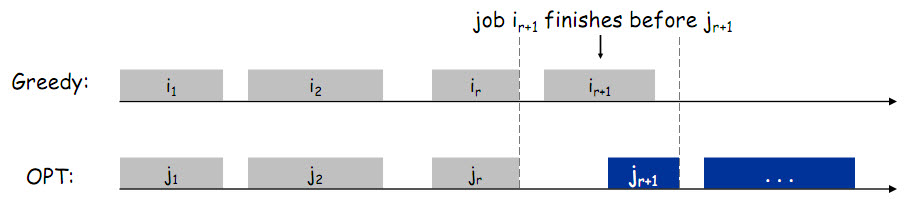
\includegraphics[height=1in]{example-hw-image.jpg}
 \caption{Comparing two sets of jobs}
\end{figure}

\subsection{This part has an example of writing algorithm psuedocode.}
Assume that there are $n$ jobs and the $\ord{i}$ job has a
start time $s(i)$ and a finish time $f(i)$. These jobs are sorted with
respect to their finish time.
For simplicity, we assume that the sorted jobs are numbered 1,2,...,
$n$ such that $f(1)\leq f(2)\leq \cdots \leq f(n)$.

A set of jobs is \emph{compatible} with a job $j$
if none of the jobs in the set overlaps with $j$.
The algorithm maintains $A$, a set of selected jobs,
which is initially empty.
Our intuitive approach is to grow $A$ by choosing a compatible job
with the earliest finish time at each step.

\begin{algorithm}
\SetKwInOut{Input}{input}\SetKwInOut{Output}{output}
\DontPrintSemicolon
\Input{a list $L$ of $n$ jobs.}
\Output{a maximum set of mutually compatible jobs.}
\BlankLine
\nl Sort jobs by finish times so that $f(1) \leq f(2) \leq \cdots \leq f(n)$.\;
\nl Maintain a set \(A\) which is initially empty.\;
\nl    \For{ $i = 1$ \KwTo $n$}{
\nl    If the job $i$ is compatible with $A$, then include $i$ to $A$.}
\nl Output $A$.
\caption{Earliest-Finish-Time(\(L\)).\label{alg:earliest-finish-time}}
\end{algorithm}



Let $i_1,...,i_k$ be the set of jobs in $A$ in the order they were
added to $A$. Similarly, let the set of jobs in $B$, which selects
jobs in some method other than greedy approach, be denoted by
$j_1,...,j_\ell$.
One interesting consequence is that the greedy rule \emph{stays ahead}:
$f(i_m)\leq f(j_m)$ for $1\leq m\leq \min(k, \ell)$.
\vspace{.1in}
\begin{claim}
  For all indices $m\leq \min(k,\ell)$, $f(i_m)\leq f(j_m)$.
  \label{claim:stay_ahead}
\end{claim}
\begin{proof}
  We prove by induction on the index $m$.
  For $m=1$, the statement is true because the greedy approach selects
  the job with the earliest finish time.
  For $m>1$, we will assume the statement is true for $m=t-1$ and
  prove it for $m=t$. The $\ord{t}$ job in $B$ must start after
  $f(j_{t-1})$ since this job is compatible with $B$. It means
  $f(j_{t-1})\leq s(j_t)$. By combining the induction hypothesis
  $f(i_{t-1})\leq f_j(t-1)$, it also means $f(i_{t-1})\leq s(j_t)$.
  So this job is compatible with $A$ too.
  As the greedy algorithm selects a job with earliest finish time,
  $f(i_t)$ is not larger than $f(j_t)$.
  This completes the induction step; therefore, the statement is true.
\end{proof}
\paragraph{Proof of Correctness}
Assume for contradiction that the greedy approach returns a
non-optimal solution $A$ while an optimal set $\Ocal$ has more
jobs. Assume that $|A|=k$ and $|\Ocal|=\ell$ with $\ell > k$.
By Claim \ref{claim:stay_ahead}, we have $f(i_k)\leq f(j_k)$.
Let us focus on the $\ord{(k+1)}$ job $x$ in $\Ocal$. The job $x$ starts
after the job $j_k$ ends and hence after the job $i_k$ ends.
But the greedy algorithm stops with $i_k$ while $x$ is compatible with
$A$ -- a contradiction.

\paragraph{Implementation}
Once the input jobs are sorted, an array is enough for the set $A$.
When a new job is checked for compatibility with $A$, it is
enough to compare its start time with the last added job $x$'s finish time rather
than all the jobs' finish  times in
$A$ -- the resource becomes free after $f(x)$ and the input jobs are
sorted.

\paragraph{Time and Space Complexity}
It takes $\Theta(n \log n)$ time to sort the input jobs of size $n$.
Creating an array of size $n$ takes $O(n)$ time.
For each job, it takes $O(1)$ time to check whether a job is
compatible with the set $A$, and the array can be updated in
constant time if we maintain an end-of-the-array pointer.
These operations must be repeated for each job, so the \texttt{For}
loop takes $O(n)$ time. Hence, the total running time is
$O(n\log n)$.

It takes $O(n)$ space to store the input. An in-place
sorting takes $O(n)$ space. Finally, the set $A$ can be implemented
by an array of size $n$. Thus, the space complexity is $O(n)$.
\end{document} 